\documentclass[a4paper, twocolumn, superscriptaddress,prl]{revtex4}  %% REVTeX 4.0
\usepackage{graphicx}
\usepackage{amsmath,amssymb,braket}

\begin{document}
\title{Quantum enhanced fluorescence microscopy with a single photon avalanche diode array}
\author{Clayton Seitz}
\affiliation{Department of Physics, Indiana University, Indianapolis}

\begin{abstract}
Localization microscopy uses precise localization of isolated fluorescent emitters to produce super-resolved images. The number of fluorescent emitters is a critical piece of information during localization, which cannot be reliably estimated with conventional microscopies. Photon statistics can enable localization in non-sparse scenes by providing information on the number of active fluorescent emitters. This work introduces a model for accurately counting active fluorescent emitters, demonstrated using a single photon avalanche diode (SPAD) array. SPAD cameras, with their high temporal resolution and single photon sensitivity, offer significant advantages for widefield imaging. Integrating photon statistics with conventional super-resolution techniques may enhance bioimaging capabilities, building on previous methods utilizing small detector bundles and laser scanning.
\end{abstract}

\maketitle 

\subsection{Introduction}

Far-field optical microscopy is fundamentally limited by diffraction, with the maximum attainable resolution being limited to approximately half the wavelength of light. Several schemes to beat the diffraction limit have been developed in recent years. Many of these schemes utilize the concept of precise localization of isolated fluorescent emitters which blink over a time series of frames. An inherent problem with such methods is the requirement that fluorescent emitters be isolated, slowing down the acquisition of super-resolved images. To address this, gathering additional information on the number of active emitters by computing photon correlation statistics can potentially enable localization in non-sparse scenes. 

Molecular counting with photon statistics has a fairly simple motivation: coincidence of photons at multiple detector elements during high speed imaging provides evidence for the number of emitters present in the imaged region. Combining the ideas of conventional super-resolution approaches, with photon statistics may prove to be a powerful set of methods for bioimaging. Indeed, single photon arrays technologies, such as SPAD cameras with orders of magnitude higher temporal resolutions than standard CMOS cameras, single photon sensitivity, and theoretically zero readout noise have already begun to be integrated into fluorescence microscopes (Forbes 2019). Furthermore, the reduced readout noise and large fill-factor of the SPAD array suggests its use for single molecule localization with reduced localization uncertainty. Localization uncertainty, typically the RMSE of a maximum likelihood or similar statistical estimator, is bounded from below by the inverse of the Fisher information matrix, known as the Cramer-Rao lower bound (Chao 2016). Managing the increase in localization uncertainty at high labeling density remains a major bottleneck to SMLM. For example, static uncertainty due to molecular crowding can be partially amelioriated by using pairwise or higher-order temporal correlations within a pixel neighborhood (Dertinger 2009). However, the number of fluorescent active emitters in a region of interest remains critical prerequisite information in their application.

In this study, we present a method for widefield single photon counting in order to rigorously count fluorophores in the sample and subsequently constrain single molecule localization. We investigate the theoretical properties of the zero-lag second-order coherence function $g^{(2)}(0)$ for widefield photon counting and its spatial properties. Using Bayesian analysis, we derive a posterior distribution on the number of active fluorescent emitters in a region of interest. We then combined this with single molecule localization algorithms and demonstrate resolution of multiple emitters using a multi-emitter fitting algorithm and report localization errors with respect to the Cramer-rao lower bound.

\subsection{Basic Scheme}

\begin{figure*}
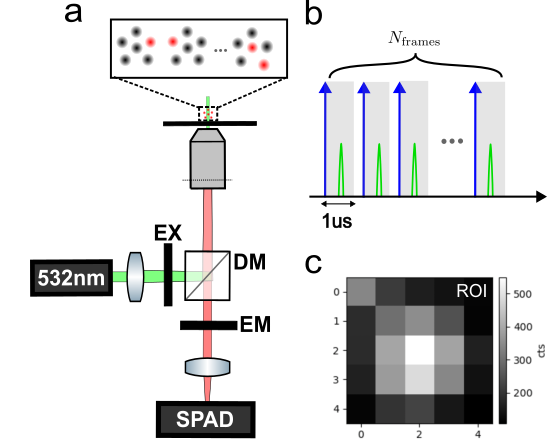
\includegraphics[width=14cm]{Figure-0.png}
\caption{Single photon counting with a SPAD array (a) Conventional widefield microscopy with integrated SPAD array (b) Single photon imaging scheme using 1us exposures containing a picosecond laser pulse (c) Sum of photon counts over a 5x5 region of interest (ROI), taken with $N_{\mathrm{frames}}=5\times 10^{5}$}
\end{figure*}    

We consider a simplified description of widefield photon counting for a a single photon source in the object plane labeled by a continuous-valued coordinate $r=(x,y)$. The point-spread function $O$ of the field in object space to image space is presumed to have a Gaussian shape (Zhang 2007)

\begin{equation}
O(s-r) = \frac{1}{\sigma\sqrt{2\pi}}\exp\left(-\frac{(s-r)^2}{2\sigma^2}\right)
\end{equation}

The field operator in object space is $\hat{E}(r) \propto \hat{a}$ and in image space $\hat{E}(s) \propto O(s-r)\hat{a}$. Since our SPAD detectors at the image plane must be discrete, the total field at a detector element $i$ centered in image space at $s_n=(u_n,v_n)$ is then given by

\begin{equation}
\hat{E}(s_i) \propto \int d^{2}s O(s-r)\hat{a}
\end{equation}

where $\int d^2 s \; O(s-r) = \frac{1}{2}\lambda_{x}(x) \lambda_{y}(y)$ where, for example,

\begin{align*}
\lambda_{x}(x) = \frac{1}{\sqrt{2}}\left(\mathrm{erf}\left(\frac{u_i+\frac{1}{2}-x}{\sqrt{2}\sigma}\right) -\mathrm{erf}\left(\frac{u_i-\frac{1}{2}-x}{\sqrt{2}\sigma}\right)\right)
\end{align*}

We consider the case of pulsed excitation where the interval between pulses much longer than the fluorescence lifetime. Upon excitation of an isolated fluorescent emitter, a photon is detected at a particular detector element $n$ with probability $\zeta\propto \langle \hat{E}^{\dagger}(s_i)\hat{E}(s_i)\rangle = \frac{1}{4}\lambda_{x}^2 \lambda_{y}^2\mathrm{Tr}(\rho a^{\dagger}a)$ where $\rho$ is the density matrix for a two-level system. Similarly, the probability of detection in a region of interest collecting all photons emitted is $\zeta\propto \mathrm{Tr}(\rho a^{\dagger}a)$. Here, we are primarily concerned with the latter quantity, and its application in counting fluorescent emitters.

\begin{figure*}
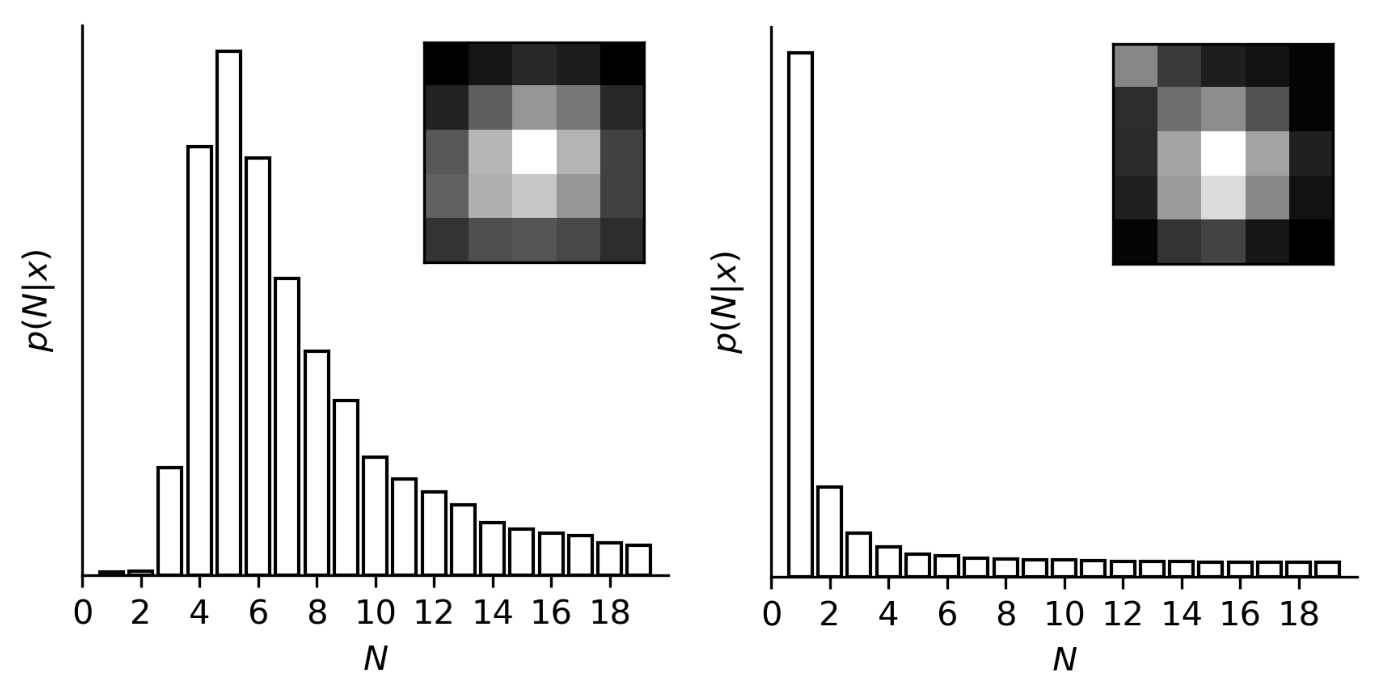
\includegraphics[width=15cm]{Figure-4.png}
\caption{Single molecule localization with a SPAD array. (a) Posteriors on the number of fluorescent emitters and localization of one and two quantum dots (b) Localization uncertainty for simulated data}
\end{figure*}   

For $N$ fluorophores emitting photons which can be detected within a region of interest of the SPAD array, the number of photons emitted $n$ following a single excitation pulse will have Binomial statistics $n_{\mathrm{signal}} \sim \mathrm{Binom}(N,\zeta)$. The probability of photon pile-up at a single detector element is neglected. We model the background signal at each detector element within the region of interest as a coherent state, which must follow Poissonian statistics $n_{\mathrm{background}} \sim \mathrm{Poisson}(\lambda)$. The total number of counts $n$ is then distributed by the likelihood

\begin{equation}
p(n=k \mid N, \zeta) = \sum_{i=0}^{\infty} \binom{N}{i} \zeta^i (1-\zeta)^{N-i} \frac{\lambda^{k-i}}{(k-i)!} e^{-\lambda}
\end{equation}

The likelihood in (2) can be used to model photon arrivals measured by the array.


\subsection{Results}

 
Fluorophores were excited using a picosecond $532\mathrm{nm}$ pulsed laser triggered at $500\mathrm{kHz}$. Emission light was collected using an oil-immersion 100$\times$ objective with numerical aperture (NA) 1.4 (Nikon). The emission signal was then filtered to exclude the laser line (Semrock) and projected onto the SPAD512 sensor (Pi Imaging Technologies) using a tube lens. A simplified diagram of the complete system is depicted in (Figure 1a). Each acquisition consists of $N=5\times 10^{5}$ frames (500ms), synchronized with each laser pulse, using a $1\mathrm{us}$ exposure per frame (Figure 1b). Using this scheme, we then investigated properties of the zero-lag second order coherence function $g^{(2)}(0)$, using quantum dots coated on a glass coverslip (Figure 1d,e). The following empirical estimate of $g^{(2)}(0)$ is used (Israel 2017)

\begin{equation}
g^{(2)}(0) = \frac{G^{(2)}(0)-B}{\langle G^{(2)}(m)\rangle -B}
\end{equation}

where $B = N_{\mathrm{frames}}\lambda\zeta$ is the expected number of background-signal coincidences in the region of interest. The quantity $G^{(2)}(m)$ represents the number of signal-signal coincidences in the region of interest at a lag time $m$, and is also binomially distributed $G^{(2)}(m)\sim \mathrm{Binom}(N_{\mathrm{frames}},\zeta_{m})$.

In order to perform localization for fluorophores which are not necessarily isolated, we write a posterior distribution on the Binomial parameters used in the likelihood (2) using Bayes rule

\begin{equation*}
\log p(N,\zeta|x) = \log p(x|N,\zeta) + \log p(\zeta) + C
\end{equation*}

where $C$ is an arbitrary constant. We use a Gaussian prior on $\zeta$ i.e., $p(\zeta) = \mathcal{N}(\mu_{\zeta},\sigma_{\zeta})$. This posterior can be integrated over $\zeta$ to produce a posterior distribution on the fluorophore number $N$ i.e., $p(N=n|x) \propto \int_{0}^{1} \prod_{j} p(x_{j}|n,\zeta)p(\zeta) d\zeta$ which is estimated via Monte Carlo integration. The final posterior is then estimated by minibatching the data into batches of $10^3$ frames and averaging the posterior $p(N|x)$ over minibatches.

It is instructive to now combine (1,3) to form a likelihood on the sum of counts at each pixel in a region of interest. Such a likelihood is Poisson, as the background is modeled as shot noise, and the signal is well approximated by a Poisson distribution for a large frame number. Denoting the fluorophore coordinates by $\theta$ and vector of total counts in the region of interest $\vec{n}$, we have the following log-likelihood

\begin{align}
\ell(\vec{n}|\theta) &= -\log \prod_{k} \frac{e^{-\left(\mu_{k}\right)}\left(\mu_{k}\right)^{n_{k}}}{n_{k}!}\\
&= \sum_{k}  \log n_{k}! + \mu_{k} - n_{k}\log\left(\mu_{k}\right)
\end{align}

where, in the multi-emitter regime the expected photon count at each pixel is $\mu_{k} = \sum_{m=1}^{N^{*}} \mu_{k,m}$ given the maximum aposteriori (MAP) estimate of the fluorophore number $N^{*}$. We then use Goodman and Weare's Markov Chain Monte Carlo (MCMC) algorithm to sample from the posterior on fluorophore locations. Fluorophore locations and their uncertainty can then be identified by taking clustering the posterior samples into modes (Figure 2). 

We now claim that the mean of each identified of posterior cluster is a efficient and unbiased estimator of fluorophore locations. The Poisson log-likelihood (5) is convenient for computing the Fisher information matrix for $\theta$ and thus the Cramer-Rao lower bound, which bounds the variance of a statistical estimator of $\theta$, from below (Chao 2016). The Fisher information is (Smith 2010)

\begin{equation}
I_{ij}(\theta) = \underset{\theta}{\mathbb{E}}\left(\frac{\partial \ell}{\partial\theta_{i}}\frac{\partial\ell}{\partial\theta_{j}}\right) = \sum_{k}\frac{1}{\mu_{k}}\frac{\partial \mu_{k}}{\partial\theta_{i}}\frac{\partial \mu_{k}}{\partial\theta_{j}}
\end{equation}

The Cramer-Rao bound is then found by $\mathrm{var}(\theta) \geq I^{-1}(\theta)$

\subsection{Discussion}

Many fluorescent emitters exhibit random variations of brightness known as blinking. Blinking increases the observed photon-number fluctuations and could be expected to affect the value of $g^{(2)}(0)$ or the posterior on the number of active fluorescent emitters. However, the photon number will follow a Binomial statistics even in the presence of blinking, the only consequence of which is an effective reduction of the emission probability. If the effect of censoring photons by blinking and lowering the quantum yield can be accounted for, the technique used here may be compatible with common super-resolution techniques such as stochastic optical reconstruction microscopy (STORM). 

The acquisition times necessary to obtain sufficient photon counts for computing the necessary statistics can potentially be very short. Most fluorophores have relaxation times in the nanosecond range and thus photons can be collected at a rate of at tens of millions of excitation pulses per second. These rates are currently difficult to obtain, however, due to limitations in detector throughput. Current state of the art and commercially available SPAD cameras have a minimum exposure time in the microsecond range. Furthermore, the data volume can quickly become intractable due to the need for several thousands of frames for a millisecond-scale exposure time. This is currently a complication for techniques like STORM and advancements in the automation for data acquisitions are necessary. 

In conclusion, we propose a single molecule imaging technique that allows for simultaneous counting of localization of fluorescent molecules by modeling the quantum properties of fluorescence emission. The technique does not require a nonclassical light source and is designed to supplement standard single molecule localization microscopy techniques. The proposed method can be implemented with a standard widefield fluorescence microscope.



\begin{thebibliography}{31}
\expandafter\ifx\csname natexlab\endcsname\relax\def\natexlab#1{#1}\fi
\expandafter\ifx\csname bibnamefont\endcsname\relax
  \def\bibnamefont#1{#1}\fi
\expandafter\ifx\csname bibfnamefont\endcsname\relax
  \def\bibfnamefont#1{#1}\fi
\expandafter\ifx\csname citenamefont\endcsname\relax
  \def\citenamefont#1{#1}\fi
\expandafter\ifx\csname url\endcsname\relax
  \def\url#1{\texttt{#1}}\fi
\expandafter\ifx\csname urlprefix\endcsname\relax\def\urlprefix{URL }\fi
\providecommand{\bibinfo}[2]{#2} \providecommand{\eprint}[2][]{\url{#2}}

\bibitem[{\citenamefont{Fujita et~al.}(2007)}]{KawataPRL07}
\bibinfo{author}{\bibfnamefont{K.}~\bibnamefont{Fujita}} \bibnamefont{et~al.},
  \bibinfo{journal}{Phys. Rev. Lett.} \textbf{\bibinfo{volume}{99}},
  \bibinfo{eid}{228105} (\bibinfo{year}{2007}).

\bibitem[{\citenamefont{{Gustafsson}}(2005)}]{Gustafsson_SSI_PNAS05}
\bibinfo{author}{\bibfnamefont{M.~G.~L.} \bibnamefont{{Gustafsson}}},
  \bibinfo{journal}{Proc. Nat. Acad. Sci.} \textbf{\bibinfo{volume}{102}},
  \bibinfo{pages}{13081} (\bibinfo{year}{2005}).

\bibitem[{\citenamefont{Hell and Wichmann}(1994)}]{STED_Hell_OL1994}
\bibinfo{author}{\bibfnamefont{S.}~\bibnamefont{Hell}} \bibnamefont{and}
  \bibinfo{author}{\bibfnamefont{J.}~\bibnamefont{Wichmann}},
  \bibinfo{journal}{Optics Letters} \textbf{\bibinfo{volume}{19}},
  \bibinfo{pages}{780} (\bibinfo{year}{1994}).

\bibitem[{\citenamefont{Betzig et~al.}(2006)}]{PALM_Betzig_Science2006}
\bibinfo{author}{\bibfnamefont{E.}~\bibnamefont{Betzig}} \bibnamefont{et~al.},
  \bibinfo{journal}{Science} \textbf{\bibinfo{volume}{313}},
  \bibinfo{pages}{1642} (\bibinfo{year}{2006}).

\bibitem[{\citenamefont{Hess et~al.}(2006)\citenamefont{Hess, Girirajan, and
  Mason}}]{PALM_Sam_Hess_BiophysJ2006}
\bibinfo{author}{\bibfnamefont{S.}~\bibnamefont{Hess}},
  \bibinfo{author}{\bibfnamefont{T.}~\bibnamefont{Girirajan}},
  \bibnamefont{and} \bibinfo{author}{\bibfnamefont{M.}~\bibnamefont{Mason}},
  \bibinfo{journal}{Biophysical journal} \textbf{\bibinfo{volume}{91}},
  \bibinfo{pages}{4258} (\bibinfo{year}{2006}).

\bibitem[{\citenamefont{Michael J.~Rust and Zhuang}(2006)}]{STORM_NatMet06}
\bibinfo{author}{\bibfnamefont{M.~B.} \bibnamefont{Michael J.~Rust}}
  \bibnamefont{and} \bibinfo{author}{\bibfnamefont{X.}~\bibnamefont{Zhuang}},
  \bibinfo{journal}{Nature Methods} \textbf{\bibinfo{volume}{3}},
  \bibinfo{pages}{793} (\bibinfo{year}{2006}).

\bibitem[{\citenamefont{Dertinger et~al.}(2009)}]{SOFI_DertingerPNAS2009}
\bibinfo{author}{\bibfnamefont{T.}~\bibnamefont{Dertinger}}
  \bibnamefont{et~al.}, \bibinfo{journal}{Proc. Nat. Acad. Sci.}
  \textbf{\bibinfo{volume}{106}}, \bibinfo{pages}{22287}
  (\bibinfo{year}{2009}).

\bibitem[{\citenamefont{Lidke
  et~al.}(2005)}]{Localization_by_blinking_Heintzmann_OpEx2005}
\bibinfo{author}{\bibfnamefont{K.}~\bibnamefont{Lidke}} \bibnamefont{et~al.},
  \bibinfo{journal}{Optics Express} \textbf{\bibinfo{volume}{13}},
  \bibinfo{pages}{7052} (\bibinfo{year}{2005}).

\bibitem[{\citenamefont{Giovannetti et~al.}(2004)\citenamefont{Giovannetti,
  Lloyd, and Maccone}}]{Quantum_Enhanced_measurements_Science2004}
\bibinfo{author}{\bibfnamefont{V.}~\bibnamefont{Giovannetti}},
  \bibinfo{author}{\bibfnamefont{S.}~\bibnamefont{Lloyd}}, \bibnamefont{and}
  \bibinfo{author}{\bibfnamefont{L.}~\bibnamefont{Maccone}},
  \bibinfo{journal}{Science} \textbf{\bibinfo{volume}{306}},
  \bibinfo{pages}{1330} (\bibinfo{year}{2004}).

\bibitem[{\citenamefont{Brida et~al.}(2010)\citenamefont{Brida, Genovese, and
  Berchera}}]{Sub_shot_noise_imaging_NatPhot2010}
\bibinfo{author}{\bibfnamefont{G.}~\bibnamefont{Brida}},
  \bibinfo{author}{\bibfnamefont{M.}~\bibnamefont{Genovese}}, \bibnamefont{and}
  \bibinfo{author}{\bibfnamefont{I.}~\bibnamefont{Berchera}},
  \bibinfo{journal}{Nature Photonics} \textbf{\bibinfo{volume}{4}},
  \bibinfo{pages}{227} (\bibinfo{year}{2010}).

\bibitem[{\citenamefont{D'Angelo et~al.}(2001)\citenamefont{D'Angelo, Chekhova,
  and Shih}}]{Lithography_proof_of_principle_PRL2001}
\bibinfo{author}{\bibfnamefont{M.}~\bibnamefont{D'Angelo}},
  \bibinfo{author}{\bibfnamefont{M.~V.} \bibnamefont{Chekhova}},
  \bibnamefont{and} \bibinfo{author}{\bibfnamefont{Y.}~\bibnamefont{Shih}},
  \bibinfo{journal}{Phys. Rev. Lett.} \textbf{\bibinfo{volume}{87}},
  \bibinfo{pages}{013602} (\bibinfo{year}{2001}).

\bibitem[{\citenamefont{Afek et~al.}(2010)\citenamefont{Afek, Ambar, and
  Silberberg}}]{Afek_Science2010}
\bibinfo{author}{\bibfnamefont{I.}~\bibnamefont{Afek}},
  \bibinfo{author}{\bibfnamefont{O.}~\bibnamefont{Ambar}}, \bibnamefont{and}
  \bibinfo{author}{\bibfnamefont{Y.}~\bibnamefont{Silberberg}},
  \bibinfo{journal}{Science} \textbf{\bibinfo{volume}{328}},
  \bibinfo{pages}{879} (\bibinfo{year}{2010}).

\bibitem[{\citenamefont{Walther
  et~al.}(2004)}]{Four_photon_Interference_Zeilinger_Nature2004}
\bibinfo{author}{\bibfnamefont{P.}~\bibnamefont{Walther}} \bibnamefont{et~al.},
  \bibinfo{journal}{Nature} \textbf{\bibinfo{volume}{429}},
  \bibinfo{pages}{158} (\bibinfo{year}{2004}).

\bibitem[{\citenamefont{Giovannetti
  et~al.}(2009)}]{Giovannetti_Number_Resolving_PRA2009}
\bibinfo{author}{\bibfnamefont{V.}~\bibnamefont{Giovannetti}}
  \bibnamefont{et~al.}, \bibinfo{journal}{Physical Review A}
  \textbf{\bibinfo{volume}{79}}, \bibinfo{pages}{13827} (\bibinfo{year}{2009}).

\bibitem[{\citenamefont{Tsang}(2009)}]{Centroids_PRL2009}
\bibinfo{author}{\bibfnamefont{M.}~\bibnamefont{Tsang}},
  \bibinfo{journal}{Phys. Rev. Lett.} \textbf{\bibinfo{volume}{102}},
  \bibinfo{pages}{253601} (\bibinfo{year}{2009}).

\bibitem[{\citenamefont{Fonseca et~al.}(1999)\citenamefont{Fonseca, Monken, and
  P{\'a}dua}}]{deBroglie_Wavelength_Fonseca_PRL1999}
\bibinfo{author}{\bibfnamefont{E.}~\bibnamefont{Fonseca}},
  \bibinfo{author}{\bibfnamefont{C.}~\bibnamefont{Monken}}, \bibnamefont{and}
  \bibinfo{author}{\bibfnamefont{S.}~\bibnamefont{P{\'a}dua}},
  \bibinfo{journal}{Phys. Rev. Lett.} \textbf{\bibinfo{volume}{82}},
  \bibinfo{pages}{2868} (\bibinfo{year}{1999}).

\bibitem[{\citenamefont{Nogueira
  et~al.}(2001)}]{Spatial_Antibunching_Monken_PRL2001}
\bibinfo{author}{\bibfnamefont{W.~A.~T.} \bibnamefont{Nogueira}}
  \bibnamefont{et~al.}, \bibinfo{journal}{Phys. Rev. Lett.}
  \textbf{\bibinfo{volume}{86}}, \bibinfo{pages}{4009} (\bibinfo{year}{2001}).

\bibitem[{\citenamefont{Muthukrishnan et~al.}(2004)\citenamefont{Muthukrishnan,
  Scully, and
  Zubairy}}]{Quantum_microscopy_using_photon_correlations_Muthukrishnan_JOB200%
4}
\bibinfo{author}{\bibfnamefont{A.}~\bibnamefont{Muthukrishnan}},
  \bibinfo{author}{\bibfnamefont{M.}~\bibnamefont{Scully}}, \bibnamefont{and}
  \bibinfo{author}{\bibfnamefont{M.}~\bibnamefont{Zubairy}},
  \bibinfo{journal}{Journal of Optics B} \textbf{\bibinfo{volume}{6}},
  \bibinfo{pages}{S575} (\bibinfo{year}{2004}).

\bibitem[{\citenamefont{Thiel et~al.}(2007)}]{Incoherent_PRL2007}
\bibinfo{author}{\bibfnamefont{C.}~\bibnamefont{Thiel}} \bibnamefont{et~al.},
  \bibinfo{journal}{Phys. Rev. Lett.} \textbf{\bibinfo{volume}{99}},
  \bibinfo{pages}{133603} (\bibinfo{year}{2007}).

\bibitem[{\citenamefont{Kimble et~al.}(1977)\citenamefont{Kimble, Dagenais, and
  Mandel}}]{Antibunching_Kimble_PRL1977}
\bibinfo{author}{\bibfnamefont{H.}~\bibnamefont{Kimble}},
  \bibinfo{author}{\bibfnamefont{M.}~\bibnamefont{Dagenais}}, \bibnamefont{and}
  \bibinfo{author}{\bibfnamefont{L.}~\bibnamefont{Mandel}},
  \bibinfo{journal}{Phys. Rev. Lett.} \textbf{\bibinfo{volume}{39}},
  \bibinfo{pages}{691} (\bibinfo{year}{1977}).

\bibitem[{\citenamefont{Walls and
  Zoller}(1981)}]{Reduced_Fluctuations_Zoller_PRL1981}
\bibinfo{author}{\bibfnamefont{D.~F.} \bibnamefont{Walls}} \bibnamefont{and}
  \bibinfo{author}{\bibfnamefont{P.}~\bibnamefont{Zoller}},
  \bibinfo{journal}{Phys. Rev. Lett.} \textbf{\bibinfo{volume}{47}},
  \bibinfo{pages}{709} (\bibinfo{year}{1981}).

\bibitem[{\citenamefont{Mandel}(1979)}]{Sub-Poissonian_Mandel_OL1979}
\bibinfo{author}{\bibfnamefont{L.}~\bibnamefont{Mandel}},
  \bibinfo{journal}{Opt. Lett.} \textbf{\bibinfo{volume}{4}},
  \bibinfo{pages}{205} (\bibinfo{year}{1979}).

\bibitem[{\citenamefont{Brouri
  et~al.}(2000)}]{Antibunching_Diamonds_Brouri_OL2000}
\bibinfo{author}{\bibfnamefont{R.}~\bibnamefont{Brouri}} \bibnamefont{et~al.},
  \bibinfo{journal}{Opt. Lett.} \textbf{\bibinfo{volume}{25}},
  \bibinfo{pages}{1294} (\bibinfo{year}{2000}).

\bibitem[{\citenamefont{Lounis et~al.}(2000)}]{Antibunching_Alivisatos_CPL2000}
\bibinfo{author}{\bibfnamefont{B.}~\bibnamefont{Lounis}} \bibnamefont{et~al.},
  \bibinfo{journal}{Chem. Phys. Lett.} \textbf{\bibinfo{volume}{329}},
  \bibinfo{pages}{399} (\bibinfo{year}{2000}).

\bibitem[{\citenamefont{Patrick~Ambrose
  et~al.}(1997)}]{Antibunching_dye_room_temperature_Patrick_CPL1997}
\bibinfo{author}{\bibfnamefont{W.}~\bibnamefont{Patrick~Ambrose}}
  \bibnamefont{et~al.}, \bibinfo{journal}{Chem. Phys. Lett.}
  \textbf{\bibinfo{volume}{269}}, \bibinfo{pages}{365} (\bibinfo{year}{1997}).

\bibitem[{\citenamefont{Dertinger et~al.}(2010)}]{SOFI_Dertinger_OpEx_2010}
\bibinfo{author}{\bibfnamefont{T.}~\bibnamefont{Dertinger}}
  \bibnamefont{et~al.}, \bibinfo{journal}{Opt. Exp.}
  \textbf{\bibinfo{volume}{18}}, \bibinfo{pages}{18875} (\bibinfo{year}{2010}).

\bibitem[{\citenamefont{{Kendall} and {Stuart}}(1977)}]{Statistics_Kendall1977}
\bibinfo{author}{\bibfnamefont{M.}~\bibnamefont{{Kendall}}} \bibnamefont{and}
  \bibinfo{author}{\bibfnamefont{A.}~\bibnamefont{{Stuart}}},
  \emph{\bibinfo{title}{{The advanced theory of statistics. Vol.1: Distribution
  theory}}} (\bibinfo{year}{1977}).

\bibitem[{\citenamefont{Schwartz and
  Oron}(2009)}]{Pupil_Filters_Schwartz_OL2009}
\bibinfo{author}{\bibfnamefont{O.}~\bibnamefont{Schwartz}} \bibnamefont{and}
  \bibinfo{author}{\bibfnamefont{D.}~\bibnamefont{Oron}},
  \bibinfo{journal}{Opt. Lett.} \textbf{\bibinfo{volume}{34}},
  \bibinfo{pages}{464} (\bibinfo{year}{2009}).

\bibitem[{\citenamefont{Chen et~al.}(2008)}]{Nonblinking_dots_Chen_JACS2008}
\bibinfo{author}{\bibfnamefont{Y.}~\bibnamefont{Chen}} \bibnamefont{et~al.},
  \bibinfo{journal}{J. Am. Chem. Soc.} \textbf{\bibinfo{volume}{130}},
  \bibinfo{pages}{5026} (\bibinfo{year}{2008}).

\bibitem[{\citenamefont{Guerrieri
  et~al.}(2010)}]{N_photon_detection_Shapiro_PRL2010}
\bibinfo{author}{\bibfnamefont{F.}~\bibnamefont{Guerrieri}}
  \bibnamefont{et~al.}, \bibinfo{journal}{Phys. Rev. Lett.}
  \textbf{\bibinfo{volume}{105}}, \bibinfo{pages}{163602}
  (\bibinfo{year}{2010}).

\bibitem[{\citenamefont{Lita et~al.}(2008)\citenamefont{Lita, Miller, and
  Nam}}]{number_resolving_Lita_OpEx2008}
\bibinfo{author}{\bibfnamefont{A.}~\bibnamefont{Lita}},
  \bibinfo{author}{\bibfnamefont{A.}~\bibnamefont{Miller}}, \bibnamefont{and}
  \bibinfo{author}{\bibfnamefont{S.}~\bibnamefont{Nam}}, \bibinfo{journal}{Opt.
  Exp.} \textbf{\bibinfo{volume}{16}}, \bibinfo{pages}{3032}
  (\bibinfo{year}{2008}).

\end{thebibliography}

\end{document}
